\documentclass[12pt,letter]{article}

%% \usepackage[fleqn]{amsmath}
\usepackage[margin=1in]{geometry}
\usepackage{amsmath,amsfonts,amsthm,bm}
\usepackage{breqn}
\usepackage{amsmath}
\usepackage{amssymb}
\usepackage{tikz}
\usepackage{algorithm2e}
\usepackage{siunitx}
\usepackage{graphicx}
\usepackage{subcaption}
%% \usepackage{datetime}
\usepackage{multirow}
\usepackage{multicol}
\usepackage{mathrsfs}
\usepackage{fancyhdr}
\usepackage{fancyvrb}
\usepackage{parskip} %turns off paragraph indent
\usepackage{float}
\usepackage{empheq}

\pagestyle{fancy}

\usetikzlibrary{arrows}

\DeclareMathOperator*{\argmin}{argmin}
\newcommand*{\argminl}{\argmin\limits}

\newcommand{\mathleft}{\@fleqntrue\@mathmargin0pt}
\newcommand{\R}{\mathbb{R}}
\newcommand{\Z}{\mathbb{Z}}
\newcommand{\N}{\mathbb{N}}
\newcommand{\ppartial}[2]{\frac{\partial #1}{\partial #2}}
\newcommand{\norm}[1]{\|#1\|}
\newcommand{\set}[1]{\{#1\}}
\newcommand{\notimplies}{\;\not\!\!\!\implies}

\setcounter{MaxMatrixCols}{20}

\begin {document}

  % \begin{cases}
  %     0, & \text{if}\ a=1 \\
  %     1, & \text{otherwise}
  %   \end{cases}

\lhead{Convex Optimization - HW2}
\rhead{(Bill) Yuan Liu, 996954078, 2020/02/22}

\begin{enumerate}
\item Q 4.11(a,c,e) textbook\\
  (a) Minimize $\norm{Ax-b}_{\infty}$
    \begin{align*}
      \min \max_i |(Ax-b)_i|\\
      \text{let } t = max_i |(Ax-b)_i|\\
      \min_{x,t} t, subject\ to:\\
      |(Ax-b)_i| \leq t, \forall i
    \end{align*}
    LP Formulation:
    \begin{align*}
      x \in R^n, t \in R\\
      \min_{x,t} t, subject\ to.:\\
      A_{i,:}x - t \leq b_i, \forall i\\
      -A_{i,:}x - t \leq - b_i, \forall i
    \end{align*}
  (c) Minimize $\norm{Ax-b}_1, \norm{x}_{\infty} \leq 1$
    \begin{align*}
      \min_x \sum_i |(Ax-b)_i|, subject\ to:\\
      |x_i| \leq 1, \forall i\\
      let\ t_i=|(Ax-b)_i|\\
      \min_{x,t} \sum_i t_i, subject\ to:\\
      |(Ax-b)_i| \leq t_i, \forall i\\
      |x_i| \leq 1, \forall i
    \end{align*}
    LP Formulation:
    \begin{align*}
      x \in R^n, t \in R^n\\
      \min_{x,t} 1^T t, subject\ to:\\
      A_{i,:}x - t_i \leq b_i\\
      -A_{i,:}x - t_i \leq -b_i\\
      x_i \leq 1, \forall i\\
      -x_i \leq 1, \forall i\\      
    \end{align*}
    
    \pagebreak
    
    (e) Minimize $\norm{Ax-b}_1 + \norm{x}_{\infty}$
    \begin{align*}
      let\ t_i = |Ax-b|_i\\
      let\ v = max |x_i|\\
      \min_{t,v,x} \sum_i t_i + v, subject\ to:\\
      |x_i| \leq v, \forall i\\
      |Ax-b|_i \leq t_i, \forall i
    \end{align*}
    LP formulation:
    \begin{align*}
      x, t \in R^n, v \in R\\
      \min_{t,v,x} 1^T t + v, subject\ to:\\
      x_i - v \leq 0, \forall i\\
      -x_i - v \leq 0, \forall i\\
      A_{i,:}x -  t_i \leq + b_i, \forall i\\
      -A_{i,:}x - t_i \leq - b_i, \forall i\\
    \end{align*}

\item Q 4.16 textbook
  \begin{align*}
    x(t) \in \R^n, t \in \{0,..,N\}\\
    u(t) \in \R, t \in \{0,..,N\}\\
    x(t+1) = Ax(t) + bu(t), t \in \{0,..,N\}\\
    given:\\
    A\in\R^{n \times n}\\
    b \in \R^n\\
    x(0) = 0\\
    problem:\\
    \min_u \sum_{t=0}^{N-1} f(u(t)), subject\ to:\\
    X(N) = x_{des}\\
    f(a) = 
    \begin{cases}
      |a|, & |a| leq 1\\
      2|a| - 1, & |a| > 1\\
    \end{cases}\\
  \end{align*}
  
  \pagebreak
  
  expanding\ $x(t)$:\\
  \begin{align*}
    x(0)&=0\\
    x(1)&=Ax(0)+bu(0) = bu(0)\\
    x(2)&=Ax(1)+bu(1)=A(bu(0))+bu(1)\\
    x(3)&=Ax(2)+bu(2)=A(A(bu(0))+bu(1))+bu(2)\\
    x(i)&=A^{i-1}bu(0) + A^{i-2}bu(1) + ... + A^0 bu(i-1)=\sum_{j=0}^{i-1} A^{j}bu(i-1-j)\\
    x(i)&=
    \begin{bmatrix}
      A^{i-1}b & A^{i-2}b & .. & .. b
    \end{bmatrix}
    \begin{bmatrix}
      u(0) \\ .. \\ u(i-1)
    \end{bmatrix}\\
    x_{des} & = x(N) = \begin{bmatrix}
      A^{N-1}b & A^{N-2}b & .. & .. b
    \end{bmatrix}
    \begin{bmatrix}
      u(0) \\ .. \\ u(N-1)
    \end{bmatrix}\\
    let\ v_t & = |f(x(t))|\\
    v_t & = max\{ |u(t)|, 2|u(t)|-1 \}\\
    v_t &\geq |u(t)|\\
    v_t &\geq 2|u(t)|-1\\
    v_t &\geq u_t\\
    v_t &\geq -u_t\\
    v_t &\geq 2u_t-1\\
    v_t &\geq -2u_t-1
  \end{align*}
  LP formulation:
  \begin{align*}
    v_{0,..,N-1},u_{0,..,N-1} \in \R^N\\
    \min_{v,u} 1^T v, subject\ to:\\
    -v_t + u_t & \leq 0, \forall t \in {0,..,N-1}\\
    - v_t -u_t & \leq 0, \forall t \in {0,..,N-1}\\
    -v_t + 2u_t & \leq 1, \forall t \in {0,..,N-1}\\
    -v_t - 2u_t & \leq 1, \forall t \in {0,..,N-1}\\
    \begin{bmatrix}
      A^{N-1}b & A^{N-2}b & .. & .. b
    \end{bmatrix}
    \begin{bmatrix}
      u_{0} \\ .. \\ u_{N-1}
    \end{bmatrix} & = x_{des}\\
  \end{align*}
  
  \pagebreak
  
\item Q 4.21(a) textbook\\
  Find explicit solution for the QCQP:\\
  minimize $c^T x$, subject to:\\
  $x^TAx \leq 1$\\
  $A \in S^n_{++}, c \neq 0$\\

  \begin{align*}
    x^TAx & = x^TA^{1/2}A^{1/2}x = (A^{1/2}x)^T A^{1/2}x = \norm{A^{1/2}x}_2^2\\
    \norm{A^{1/2}x}_2^2 & \leq 1\\
    let\ y &= A^{1/2}x\\
    x &= A^{-1/2}y\\
    c^T x &= c^T A^{-1/2}y\\
    let\ b^T &= c^T A^{-1/2}\\
    \min b^T y &\ subject\ to:\\
    \norm{y}_2^2 & \leq 1\\
    \min b^T y & = \frac{-b^Tb \alpha }{\norm{b}}, \alpha = max \norm{y}_2 = 1\\
    y^* & = \frac{-b}{\norm{b}}\\
    x^* &= A^{-1/2}y^* = A^{-1/2} \frac{-b}{\norm{b}}\\
          & = A^{-1/2} \frac{-(c^T A^{-1/2})^T}{\norm{(c^T A^{-1/2})^T}}\\
          & = \frac{-A^{-1/2}A^{-1/2}c}{\norm{A^{-1/2} c}} = \frac{-A^{-1}c}{(c^TA^{-1} c)^{1/2}}\\
    c^Tx^* &= \frac{-c^TA^{-1}c}{(c^TA^{-1} c)^{1/2}}\\
    c^Tx^* &= -(c^TA^{-1} c)^{1/2}
  \end{align*}

  \pagebreak
  
\item Q 4.25 textbook
  
  \begin{align*}
    \varepsilon_i = \set{P_i u + q_i: \norm{u}_2 \leq 1}, i=1,..,K+L, P_i \in S^n
  \end{align*}

  Find a feasible hyperplane strictly separating $\varepsilon_1,..,\varepsilon_K$ from $\varepsilon_{K+1},..,\varepsilon_{K+L}$.
  \begin{align*}
    a^Tx+b &> 0, x \in \bigcup_{i=1}^K \varepsilon_i\\
    a^Tx+b &< 0, x \in \bigcup_{i=K+1}^{K+L} \varepsilon_i\\
    \text{let } &\epsilon > 0 \text{, a constant for strict separation}\\
    &\text{relax inequalities to:}\\
    a^Tx+b &\leq -\epsilon, x \in \bigcup_{i=1}^K \varepsilon_i\\
    a^Tx+b &\geq \epsilon, x \in \bigcup_{i=K+1}^{K+L} \varepsilon_i\\
    a^T(P_iu+q_i)+b &\leq -\epsilon, \norm{u}_2 \leq 1, i\in\{1,..,K\}\ becomes\\
    \sup_{\norm{u}_2 \leq 1} a^TP_iu + a^Tq_i + b &\leq -\epsilon, i\in\{1,..,K\}\\
    \sup_{\norm{u}_2 \leq 1} a^TP_iu &= \frac{a^TP_i (a^TP_i)^T}{\norm{a^TP_i}_2} = \norm{a^TP_i}_2\\
    \norm{a^TP_i}_2 + a^Tq_i + b &\leq -\epsilon, i\in\{1,..,K\}\\
    \norm{a^TP_i}_2 &\leq -a^Tq_i - b  -\epsilon, i\in\{1,..,K\}\\
    \\
    a^T(P_iu+q_i)+b &\geq \epsilon, \norm{u}_2 \leq 1, i=\{K+1,..,K+L\} \ becomes\\
    \inf_{\norm{u}_2 \leq 1} a^TP_iu + a^Tq_i + b &\geq \epsilon, i=\{K+1,..,K+L\}\\
    \inf_{\norm{u}_2 \leq 1} a^TP_iu &= \frac{a^TP_i (-a^TP_i)^T}{\norm{a^TP_i}_2} = -\norm{a^TP_i}_2\\
    -\norm{a^TP_i}_2 + a^Tq_i + b &\geq \epsilon, i=\{K+1,..,K+L\}\\
    \norm{a^TP_i}_2 &\leq a^Tq_i + b -\epsilon, i=\{K+1,..,K+L\}\\
  \end{align*}
  
  Second Order Cone Programming formulation:
  \begin{align*}
    &\min_{a,b}\ 0\\
    &\norm{a^TP_i}_2 \leq -a^Tq_i - b  -\epsilon, i\in\{1,..,K\}\\
    &\norm{a^TP_i}_2 \leq a^Tq_i + b -\epsilon, i\in\{K+1,..,K+L\}\\
    &\text{where } \epsilon > 0
  \end{align*}

\item Q 4.30 textbook\\
  Express as Geometric Programming:\\
  \begin{align*}
    T & \in [T_{min}, T_{max}], T_{min},T_{max} > 0 \\
    r & \in [r_{min}, r_{max}], r_{min},r_{max} > 0\\
    w & \in [w_{min}, w_{max}], w_{min},w_{max} > 0\\
    w & \leq 0.1 r\\
    T &> 0 \\
    r &> 0 \\
    w &> 0\\
    \max\ &\alpha_4 T r^2\\
    \alpha_1 \frac{T r}{w} + \alpha_2 r + \alpha_3 r w & \leq c_{max}\\
    \alpha_i &> 0, \forall i\\
  \end{align*}
  \begin{align*}
    \max\ \alpha_4 T r^2=\min\ \frac{1}{\alpha_4 T r^2} = \min\ \frac{1}{\alpha_4} T^{-1} r^{-2}\\
    \frac{\alpha_1}{c_{max}} T rw^{-1} + \frac{\alpha_2}{c_{max}} r + \frac{\alpha_3}{c_{max}} r w & \leq 1\\
    T \leq T_{max} \iff \frac{T}{T_{max}} \leq 1\\
    T \geq T_{min} \iff \frac{T_{min}}{T} \leq 1\\
    r \leq r_{max} \iff \frac{r}{r_{max}} \leq 1\\
    r \geq r_{min} \iff \frac{r_{min}}{r} \leq 1\\
    w \leq w_{max} \iff \frac{w}{w_{max}} \leq 1\\
    w \geq w_{min} \iff \frac{w_{min}}{w} \leq 1\\
    w \leq 0.1 r \iff \frac{10w}{r} \leq 1 \\    
  \end{align*}
  GP formulation:
  \begin{align*}
    \min_{T,r,w}\ \frac{1}{\alpha_4} T^{-1} r^{-2}, subject\ to:\\
    \frac{T}{T_{max}} \leq 1, \frac{T_{min}}{T} \leq 1\\
    \frac{r}{r_{max}} \leq 1, \frac{r_{min}}{r} \leq 1\\
    \frac{w}{w_{max}} \leq 1, \frac{w_{min}}{w} \leq 1\\
    \frac{10w}{r} \leq 1 \\
    \frac{\alpha_1}{c_{max}} T rw^{-1} + \frac{\alpha_2}{c_{max}} r + \frac{\alpha_3}{c_{max}} r w \leq 1\\
    given:\\
    \alpha_1,\alpha_2,\alpha_3,\alpha_4 > 0\\
    T_{min}, T_{max}, r_{min}, r_{max}, w_{min}, w_{max} > 0\\
  \end{align*}
\item Q 4.43(a-b) textbook\\
  $A:R^n \to S^m, A(x) = A_0 + x_1A_1 + .. + x_n A_n$\\
  Let $\lambda_1(x) \geq ..  \lambda_m(x)$ denote the eigenvalues of $A(x)$.\\
  Formulate problems as SDP.\\
  \begin{itemize}
  \item (a) Minimize the maximum eigenvalue\\
    SDP formulation:
    \begin{align*}
      \min_{a,x} a,\ subject\ to:\\
      A(x) \leq_{S_+^m} aI 
    \end{align*}
  \item (b) Minimize the spread of the eigenvalues
    \begin{align*}
      let\ t &= \lambda_1(x) - \lambda_m(x)\\
      \min_{t,x,a,b} t,\ & subject\ to:\\
      A(x) & \leq_{S_+^m} bI \\
      A(x) & \geq_{S_+^m} aI \\
      t - b + a & = 0
    \end{align*}
  \end{itemize}
\item reserved
\item reserved
\item Optimal Control of a Unit Mass
  \begin{itemize}
  \item a) given:
    \begin{align*}
      x(0)&=0\\
      \dot{x}(0)&=0\\
      f(t)&=p_i, i-1 < t \leq i, i=1,..,10\\
      x(10)&=1\\
      \dot{x}(10)=0\\
      minimize \sum_{i=1}^{10} p_i^2
    \end{align*}
    \begin{align*}
      let\ v &= \dot{x}\\ 
      v(i) &= v(0) + \sum_{j=0}^i \frac{f(j)}{m} = v(0) + \sum_{j=1}^i p_j, m=1\\
      v(i) &= \sum_{j=1}^i p_j = 1^T p, p \in \R^{i}\\
      v(1) &= p_1\\
      v(2) &= p_1 + p_2\\
      ...\\
      v(10) &= 1^T p = v_{des} = 0,\\
      x(i) &= x(0) + \sum_{j=0}^i v(j)\\
      x(i) &= \sum_{j=1}^i v(j) = 1^T v, v \in \R^{i}\\
      x(i) &= \sum_{j=1}^i \sum_{k=1}^j p_k\\
      x(i) &= \sum_{j=1}^i (i-j+1) p_j\\
      x(1) &= p_1\\
      x(2) &= 2 p_1 + 1p_2\\
      x(10) &= 10 p_1 + 9p_2 + .. + 1p_{10}\\
    \end{align*}
    QP formulation:
    \begin{align*}
      \min_{f} f^TIf,\ &subject\ to:\\
      \begin{bmatrix}
        & & 1^T & & \\
        10 & 9 & .. & 2 & 1
      \end{bmatrix} p &=
      \begin{bmatrix}
        0\\
        1
      \end{bmatrix}\\
      % &\text{Solve:}\\
      % f&= [0.0545, 0.0424, 0.0303, 0.0182, 0.0061,\\
      %                  &-0.0061, -0.0182, -0.0303, -0.0424 , 0.0545]
    \end{align*}
    \begin{figure}[H]
      \centering
      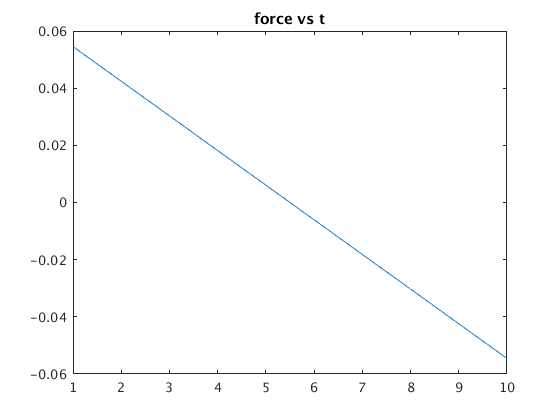
\includegraphics[width=11cm]{q9/part_a_plot_1.png}
      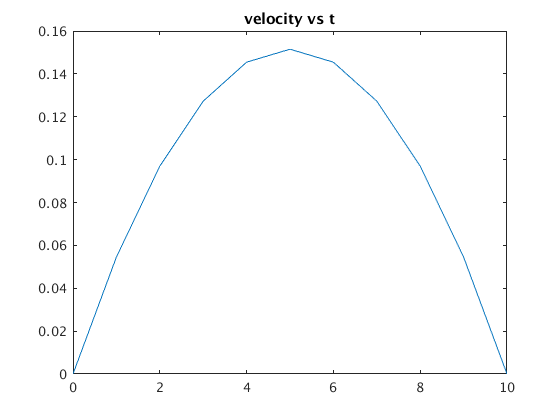
\includegraphics[width=11cm]{q9/part_a_plot_2.png}
    \end{figure}
    \begin{figure}[H]
      \centering
      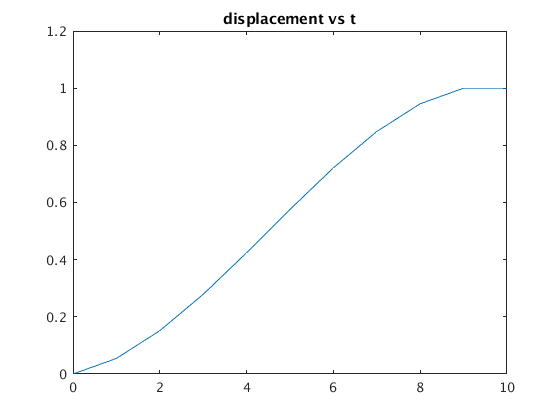
\includegraphics[width=11cm]{q9/part_a_plot_3.png}
    \end{figure}

    Optimal strategy in this case is to apply a smooth symmetrical force around t = 5, so that velocity is always non-negative and displacement is always towards the destination.
    
    \pagebreak
    
  \item b) additional constraint: $x(5) = 0$\\
    \begin{align*}
      \min_{f} f^TIf,\ &subject\ to:\\
      \begin{bmatrix}
        & & & 1^T & & & &\\
        10 & 9 & .. &&& & 2 & 1\\
        5 & 4 & 3 & 2 & 1 & 0 & .. & 0
      \end{bmatrix} p &=
      \begin{bmatrix}
        0\\
        1\\
        0\\
      \end{bmatrix}\\
      % &\text{Solve:}\\
      % f&= [-0.0471, -0.0118, 0.0235, 0.0588, 0.0941,\\
      %      &0.1294, 0.0529, -0.0235, -0.1, -0.1765]
    \end{align*}

    \begin{figure}[H]
      \centering
      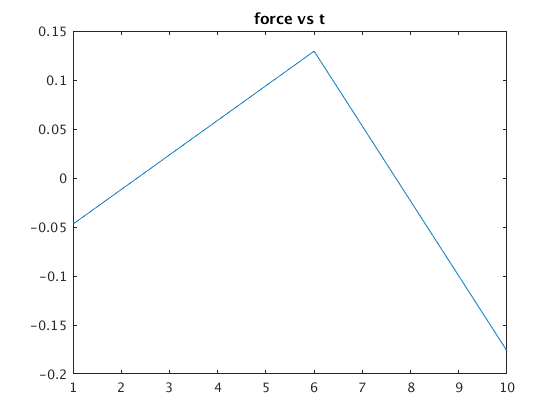
\includegraphics[width=11cm]{q9/part_b_plot_1.png}
      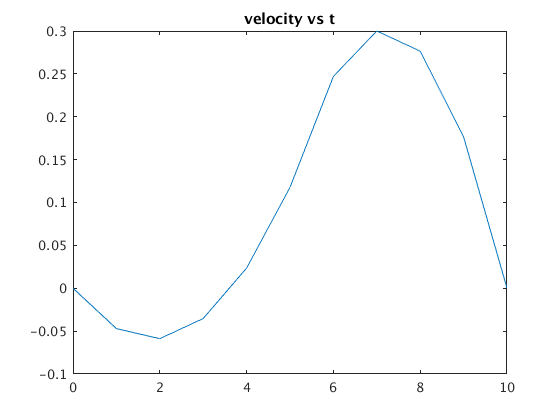
\includegraphics[width=11cm]{q9/part_b_plot_2.png}
    \end{figure}
    \begin{figure}[H]
      \centering
      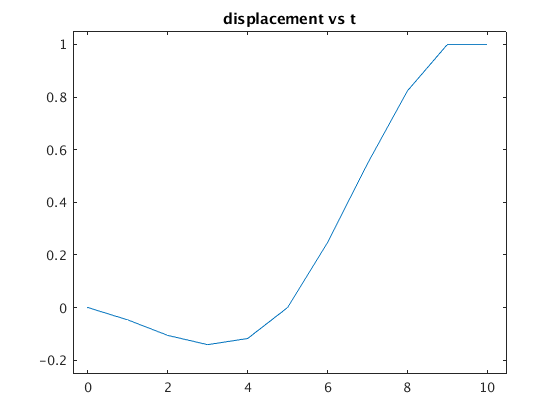
\includegraphics[width=11cm]{q9/part_b_plot_3.png}
    \end{figure}
    Optimial strategy in this case is to reverse direction and then go forward again to gain enough velocity timed so that the displacement at t=5 is 0.
  \end{itemize}
\end{enumerate}


\end {document}
